% Gene co-expression networks: https://en.wikipedia.org/wiki/Gene_co-expression_network#:~:text=Having%20gene%20expression%20profiles%20of,rise%20and%20fall%20together%20across

The cost of producing data has plummeted in recent years and many people are doing it due to technological advancement. In the field of genomics, the sequencing of the first human genome (2002) took around 13 years and cost over \$3 million to complete. Nowadays, we can sequence hundreds of genomes in just a few days with with a cost of around \$1,000 each \cite{big_biological_impacts_bd}. However, the vast amounts of data that we produce can result in a problem like data information overload. To solve this, we need new visualization tools that will help us inspect large amounts of data so that we can find novel patterns in them and this will lead to new scientific discoveries.

% These problems can be overcome with a visualization system that can scale to large sizes of data and where the interactions are not cumbersome. In this way, we can visualize the data in order to find interesting patterns that will lead to new scientific discoveries
%  \cite{zhang_paciorkowski_craig_cui_2019}.

% Some of the main problems that researchers face when analysing genomic data are: information overload, data interconnectivity and high dimensionality. One way to deal with all this data is to invent novel analysis. However, we still need visual inspection of the data, which is an important challenge, and this is what we attempt to solve. For this reason, it is very important to implement efficient visualization technologies that can lead to find new patterns and the extraction of good conclusions of the data.

In the field of system biology, there are usually network representations where the nodes or bioentities are connected to each other and where these edges represent associations. Networks can increase dramatically in size and complexity and many visualization systems for biological networks have a lack of scalability and the user interactions can be cumbersome. Virtual Reality (VR) has shown to have benefits when visualizing abstract information and offers rich interactivity \cite{zhang_paciorkowski_craig_cui_2019}. Some specific challenges that we face when visualizing biological networks in VR are the following:
\begin{itemize}
  \item Solve the problem of information overload when visualizing large biological networks in Virtual Reality.
  \item Understand the scalability limitations for the exploration of large biological networks in VR.
  \item Achieve the performance needed for the visualization of large biological networks using cheap VR equipment.
\end{itemize}

% enough computational power to create these large networks, scientific knowledge about large networks a. We need better visualization systems for the analysis and inspection of biological networks and at the same time we need robust applications that can handle the data overload.

We can find many tools for the visualization of large biological networks. Many of them are 2-dimensional, some provide a 3-dimensional view and a limited number of them are implemented for Virtual Reality. These tools struggle with information overload problems or the "hairball" effect when the network becomes larger. Some tools like Cytoscape \cite{cytoscape}, NAViGaTOR \cite{navigator} or BioLayoutExpress3D \cite{biolayout3d}, help overcome these problems with specific hardware or libraries. Other tools just trade off the interactivity in favour of showing large amounts of data \cite{agapito_guzzi_cannataro_2013}.


%[What I expect to read here is why your solution is better than the previous solutions described in the previous section.]


We have implemented GeneNet VR, a virtual reality application for the visualization of large biological networks. We used two datasets from the MIxT project \cite{dumeaux_fjukstad_interactions_tumor_blood} that contain genetic information from patients with breast cancer. MIxT provides a 2-dimensional visualization tool to explore these datasets. However, it has some known visual and scalability problems. In GeneNet VR, we overcome these problems that are common in large biological networks by providing the following solutions with GeneNet VR:
\begin{enumerate}
  \item Visualization of the network in a three-dimensional immersive space and implementation of interactive and visual solutions to reduce information overload.
  \item Use of MIxT datasets as a use case to evaluate the scalability limitations for the visualization of these type of networks.
  \item Solution implemented for the Oculus Quest, a cheap Virtual Reality headset.
\end{enumerate}

We have used the following methodology in this project: we implemented a prototype of GeneNet VR in Unity using the datasets from MIxT. Then, we evaluated performance aspects of it in both PC and in the Oculus Quest hardware. Finally, we conducted several interviews with test users where we got feedback about the quality and where we extracted some conclusions and ideas for future work.

A good performance is needed for the exploration of biological networks and for rapid pattern finding. We ran several experiments where we evaluated the performance of GeneNet VR and several of the interaction that are commonly used for network exploration. Another experiment was also carried out to evaluate the performance of the application on the Oculus Quest hardware. We concluded from the experiments that GeneNet VR has a good performance for the network sizes that we used and that the interactions with the network achieved the required Frames Per Second (FPS) defined by Oculus. We also concluded that we can use cheap VR hardware to explore biological networks. From the interviews, we received a general positive feedback, standing out that this application is helpful for the visualization of biological networks. Some problems that we didn't resolve in GeneNet VR are: a performance evaluation using larger networks; showing more information that is helpful during the exploration of the networks like the names of the interconnected genes from a selection; showing weight information in the edges; evaluate the application using similar datasets like drug networks.

\textbf{Thesis statement: } \emph{Virtual Reality is advantageous for the visualization of large biological networks and for rapid exploration of patterns in them using affordable hardware}.

\section{Challenges and research problem}

In fields like biology, network visualization seem to be particularly helpful\cite{pujana_network_modeling}\cite{fraser_view_function}. There are many types of relationships that can be measure in a biological context, for example interactions between proteins or genetic interections when revealed by combinations of mutations. All these interactions and correlations can be easier to visualize as a network\cite{merico_visualization}.

MIxT\cite{fjukstad_dumeaux_olsen_lund_hallett_bongo_2017} is a web application for bioinformaticians that is used to identify genes and pathways in the primary tumor that are tightly linked to genes and pathways in the systemic response of a patient with breast cancer\cite{dumeaux_fjukstad_interactions_tumor_blood}. Among other tools, it offers a visualization tool for the biological networks where the nodes are genes and the edges between two nodes represent a statistically significant correlation in expression between them.

OmicsNet is another example of a visualization tool with data overload problems \cite{omnicsnet}. OmicsNet is a web application to create different types of molecular interaction networks and visually explore them in a three-dimensional space. However, the application struggles with problems like edge occlusion and performance, making it hard to visualize the network when this one becomes larger.

It can be hard to identify novel patterns when exploring large amounts of data. Some data structures, like the networks, also have the challenge of data interconnectivity. These data structures represent relationships and are composed by nodes and edges. Even though we have many tools like machine learning that help researchers automatize and accelerate the finding of patterns, we still need a human expert to check and inspect these networks \cite{network_expert}.

When exploring a network in MIxT, sometimes it can be difficult to find patterns because of the data overload. This problem happens expecially when there are many nodes and relationships together. In figure \ref{fig:mixt_network} we can see an example of the network visualization from MIxT. As we can see in Figure \ref{fig:mixt_network1}, there are many nodes and relationships; this problem gets worse when we zoom in the network as in Figure \ref{fig:mixt_network_zoom}.

\begin{figure}[h!]
    \centering%
    \begin{subfigure}[t]{0.5\textwidth}
        \centering%
        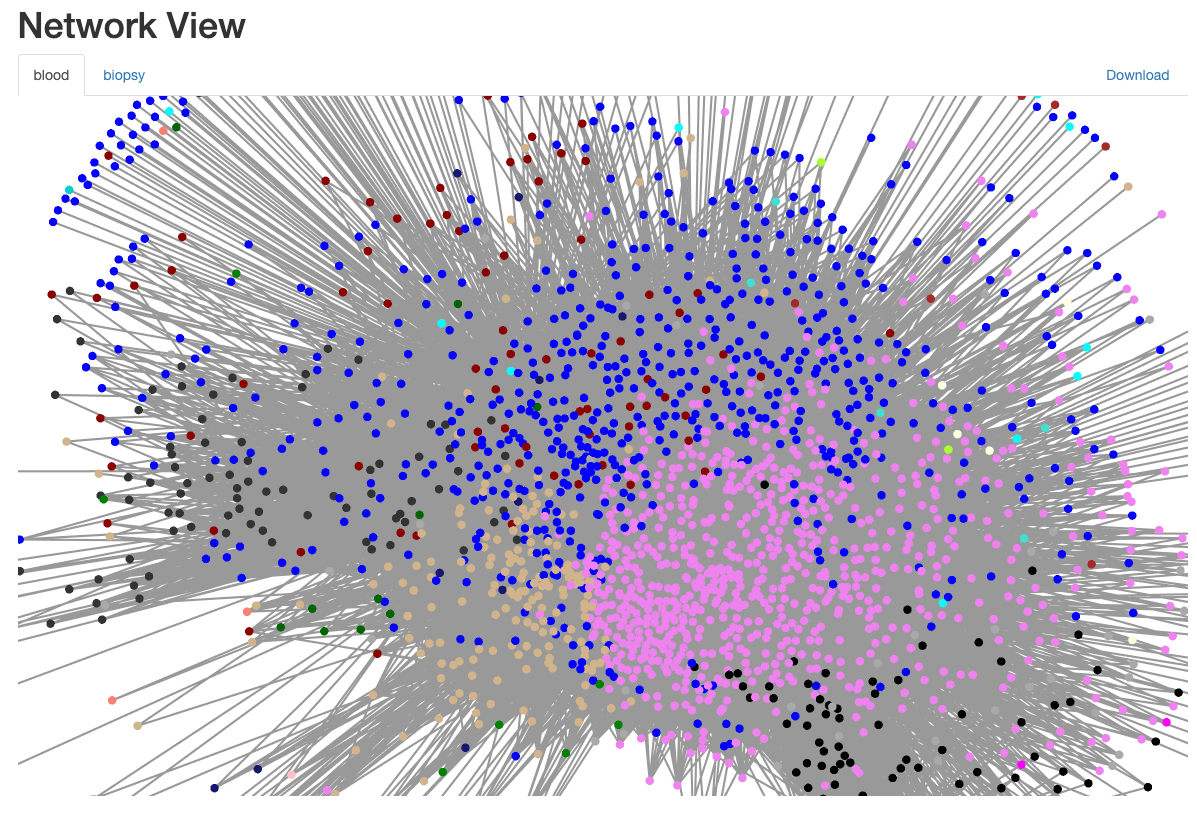
\includegraphics[width=\linewidth]{mixt_network1}
        \caption{Network with several modules.}
        \label{fig:mixt_network1}
    \end{subfigure}%
    \begin{subfigure}[t]{0.5\textwidth}
        \centering%
        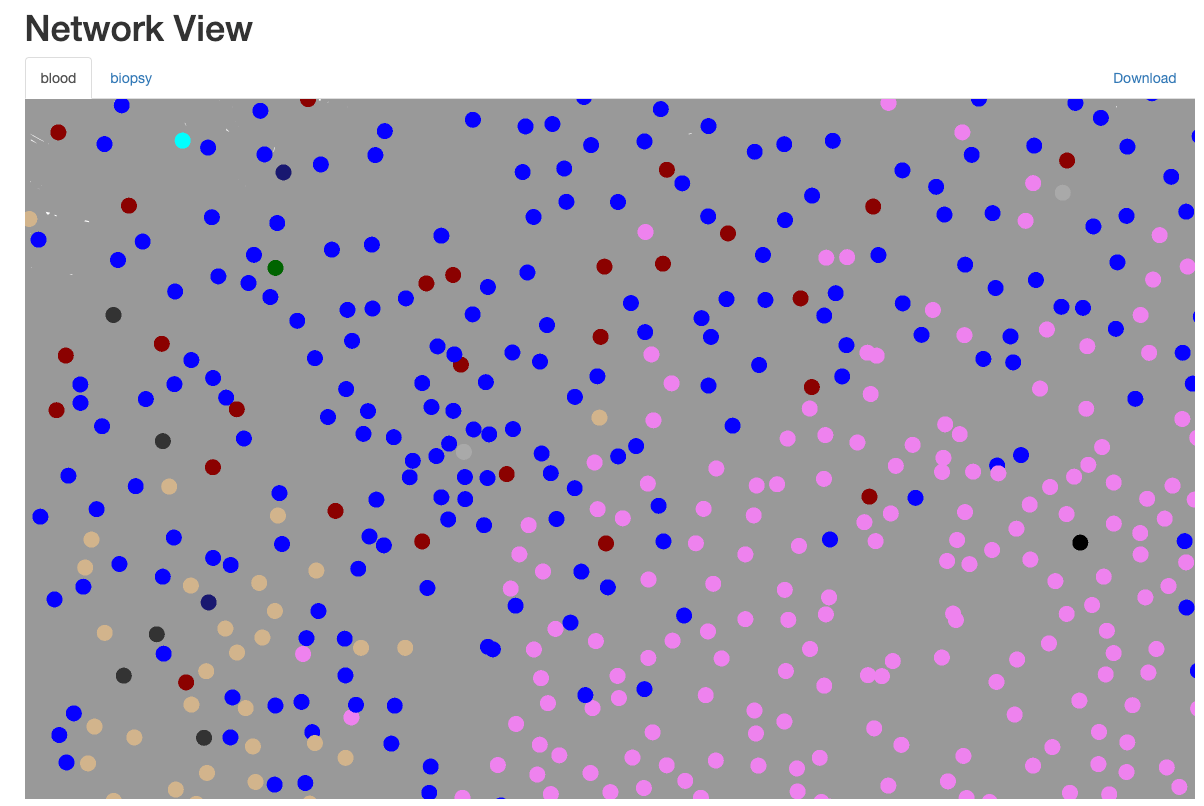
\includegraphics[width=\linewidth]{mixt_network2}
        \caption{Zoom in the network.}
        \label{fig:mixt_network_zoom}
    \end{subfigure}

    \caption{Network view of the MIxT application where nodes repsent genes and the modules are repsented by colors. Relationships are represented by grey lines that connect a gene with another one.}
    \label{fig:mixt_network}
\end{figure}

In Virtual Reality, we also have other challenges when exploring large biological networks. When we are in an immersive three-dimensional space, we have occlusion problems. This is when for example, the nodes or edges that we have in front of us, hide other nodes or edges that are behind them. A solution to this can be showing the network from other angles. We can do this by for example rotating and moving the network or by making it possible for the user to move to other parts in the virtual world. Another problem for these networks is the information overload. To solve this, we can show only the information that the user needs to visualize. This can be done, for example, by filtering the data so that we can focus on what we are interested in, or by showing just the edges and node names from the nodes that we want to explore.

The interactivity in VR is usually done with the VR controllers, which simulate our hands in the virtual world. We can implement natural actions for the human being like grabbing something with the hands, which will feel intutive. But we can also implement other actions in the virtual world like using laser pointers to select something, using 2D menus inside the virtual world or teleporting to other parts of the virtual space. In GeneNet VR, we are dealing with abstract information and the amount of data can scalate quickly if we don't implement good solutions. We need therefore to keep a good balance between the amount of data that is being visualize, comfortable and user-friendly interaction solutions for the user and a good performance.

\section{Proposed solution and contribution}

Virtual Reality offers new possibilities for visual inspection of large biological networks and for pattern finding in them. Even though VR is still a field under exploration, it has been demonstrated that it help scientists work more effectively in fields like medicine \cite{Laver11} \cite{xia_ip_samman_wong_gateno_wang_yeung_kot_tideman_2001} \cite{brain_damage_rehab}, biology \cite{bioinformatics_bti581} \cite{thorley_lawson_duca_shapiro_2008} and neuroscience \cite{bohil_alicea_biocca_2011}\cite{minderer_harvey_donato_moser_2016}, to  cite some examples.
VR is very beneficial for visualization systems because it takes advantage of the way human beings perceive and analyse information. Human beings have a great ability to discover patterns; however, they are biologically optimized to see the world and the patterns in an immersive 3-dimensional space. In addition, VR offers very rich interaction solutions. The user cannot just interact directly with the virtual world, but it is also possible to use user interfaces within the 3-dimensional world to enrich the user's experience.

Our solution, GeneNet VR, is a Virtual Reality visualization tool that focuses on solving common problems for the visualization of large biological networks. To solve the information overload problem, GeneNet VR shows the necessary information when exploring the network. The edges are shown for indevidual nodes when the user selects them. It is also possible to move around the virtual space and the user can scale or move the network for a better angle of it and to solve the occlusion problem. In addition, a filtering menu was implemented to filter the necessary information that the user wants to see. We implemented a use case where we visualize networks from biological datasets that are used in another scientific project. This helped us understand the limitations for the visualization of these type of networks. We also implemented a feature to visualize two networks at the same time, which are useful for datasets like the ones that we used.

We have also evaluated GeneNet VR, focusing on performance problems. The pattern exploration in these datasets is an important process that cannot be interrupted by slowliness and low FPS. We found out that the performance is good when visualizing datasets similar to the ones that we used in our use case. The performance was also good on the Oculus Quest headset, which is an affordable VR headset.

This project has contribuited by tracing out some the important requirements that are needed for the visualization of large biological networks in affordable Virtual Reality headsets. We could demonstrate this by implementing a prototype with a real use case. We also conducted several interviews with bioinformaticians from the University of Troms\o. This helped us corroborate the benefits of our project and also obtaine new ideas and feedback for future improvements.

GeneNet VR results in an application that offers a different way for the visualization of biological networks and that gives visualization experts interesting tools to explore biological data. In Figure \ref{fig:bignet_intro} we can see an example of GeneNet VR, where a user explores the blood dataset from MIxT. The node TMED7 is selected and its edges are shown. The user is also using a UI menu to filter the nodes.

\begin{figure}[h!]
    \newlength{\tempheight}
    \setlength{\tempheight}{15ex}
    \centering
    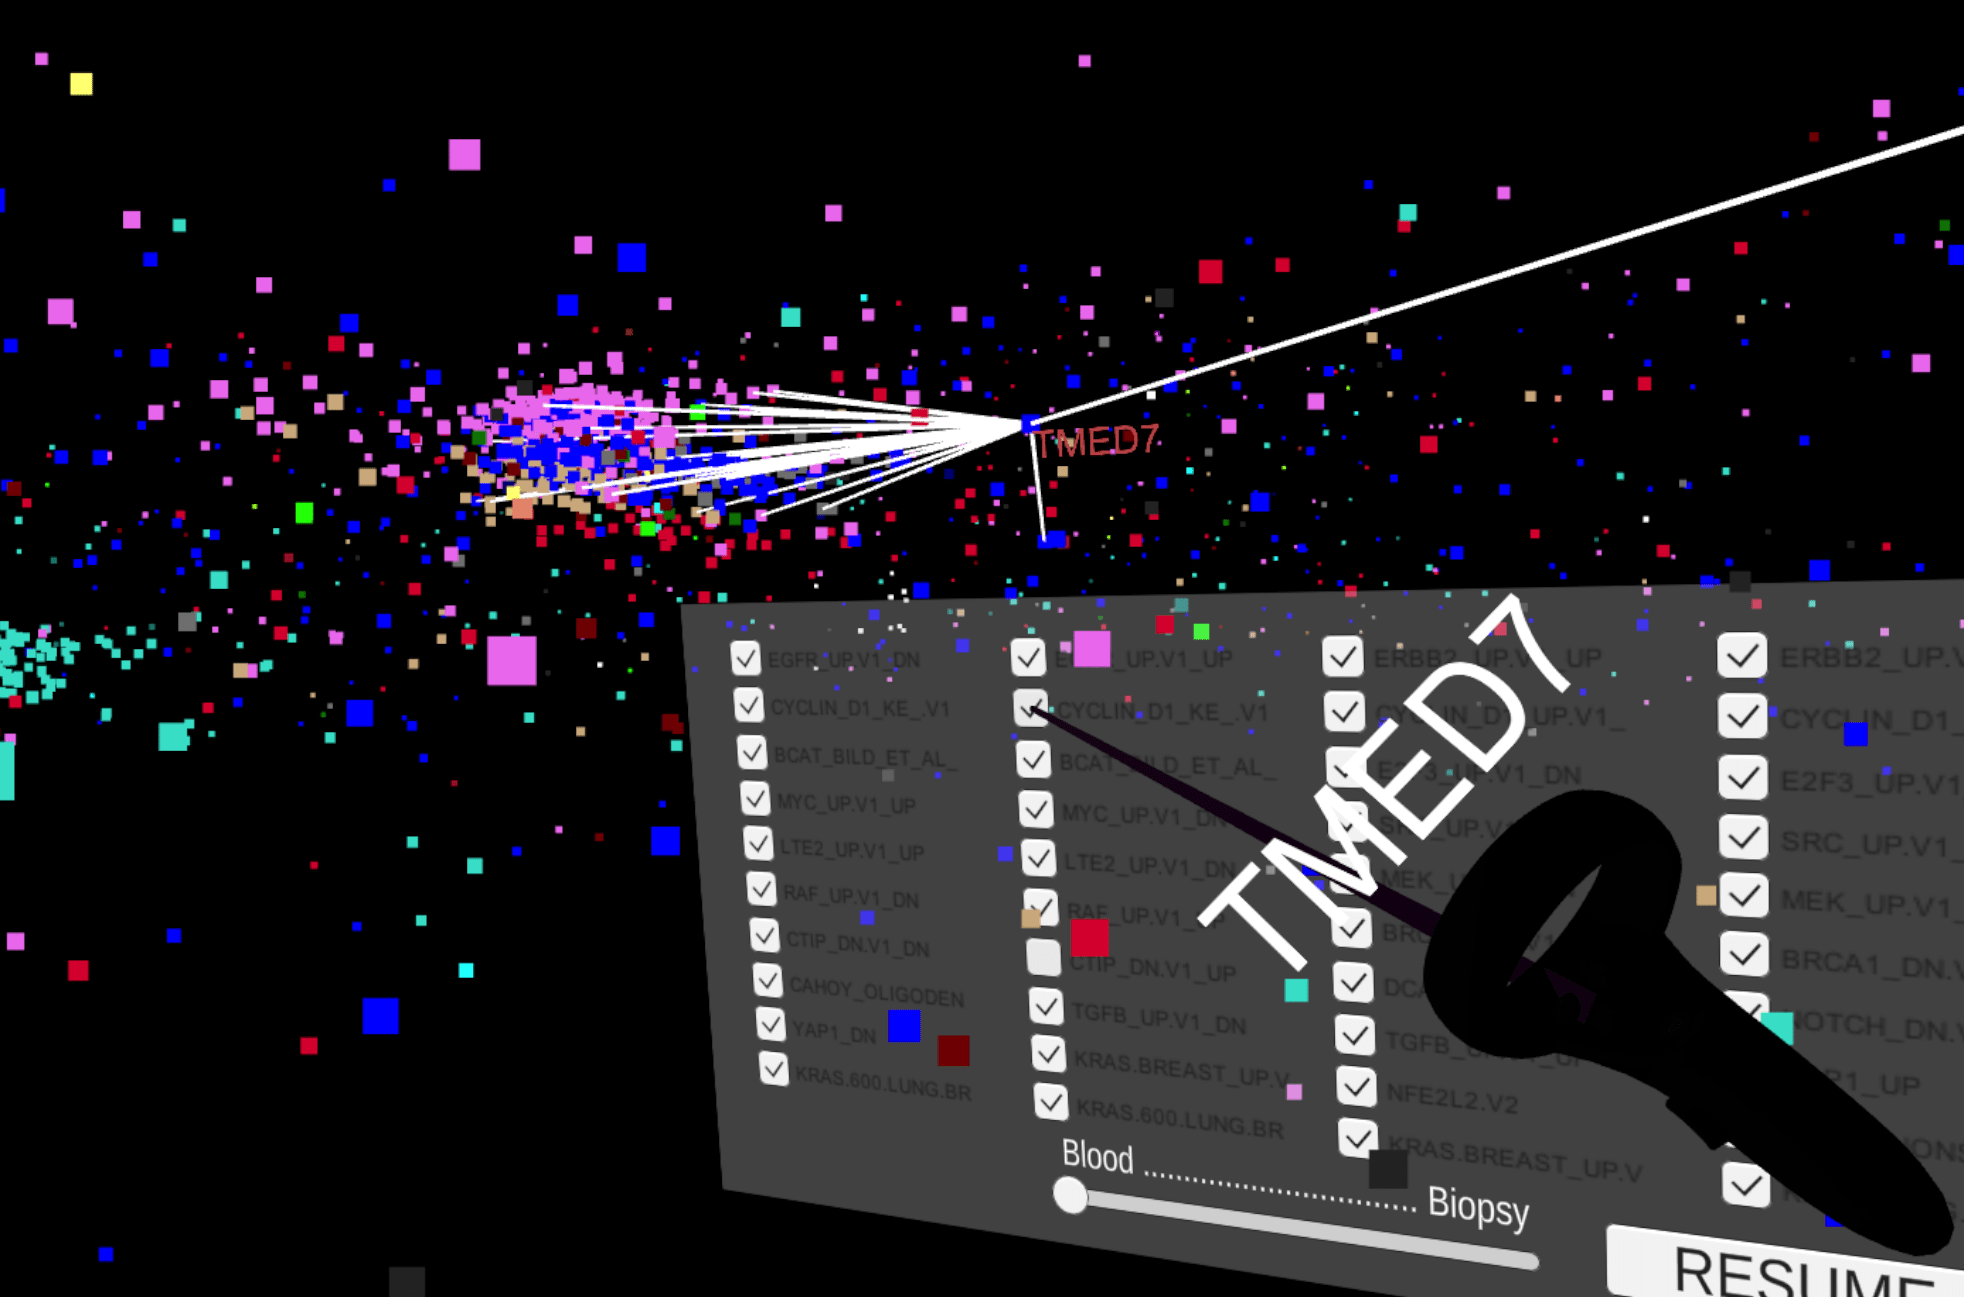
\includegraphics[width=\textwidth]{mixt_vr_introduction}
    \caption{A screenshot from GeneNet VR where a user is exploring the blood dataset from MIxT.}
    \label{fig:bignet_intro}
\end{figure}

\section{Outline}

We have structured the thesis in the following chapters: Chapter 2 descibes how GeneNet VR was implemented, the architecture, design and the Virtual Reality techniques that were used. Chapter 3 focuses on explaining the visualization of MIxT in Virtual Reality. Chapter 4 describes some related projects found in the literature and we compare them with GeneNet VR. In Chapter 5 we describe the experimens and conclusions that carried out in order to evaluate GeneNet VR. In Chapter 6 we explain the conclusions from the project. In Chapter 7 we describe the future work ideas that we have for GeneNet VR.
